This region (CR$_\mathrm{\, zmm}$) is designed to select the $\zmumuplusjets$
events in order to estimate their background contribution in the signal region
coming from this process together with the dominant $\znunuplusjets$. In
addition to cuts from A to H defined in \cref{sec:event-selection}, events in
the CR$_\mathrm{\, zmm}$ region are required to have:
\begin{itemize}
\item Exactly two good muons.
\item Electrons are vetoed.
\item An invariant mass in the $Z$ boson mass window range
  $66 < m_{\mu \mu} < 116~$GeV.
\end{itemize}
Figure~\ref{fig:dimuon_cr_plots} shows a good agreement between data and MC for
the measured $\met$ and leading jet $\pt$ distributions also in this region.
\begin{figure}[!h]
  \centering
  \begin{subfigure}[t]{.48\linewidth}
    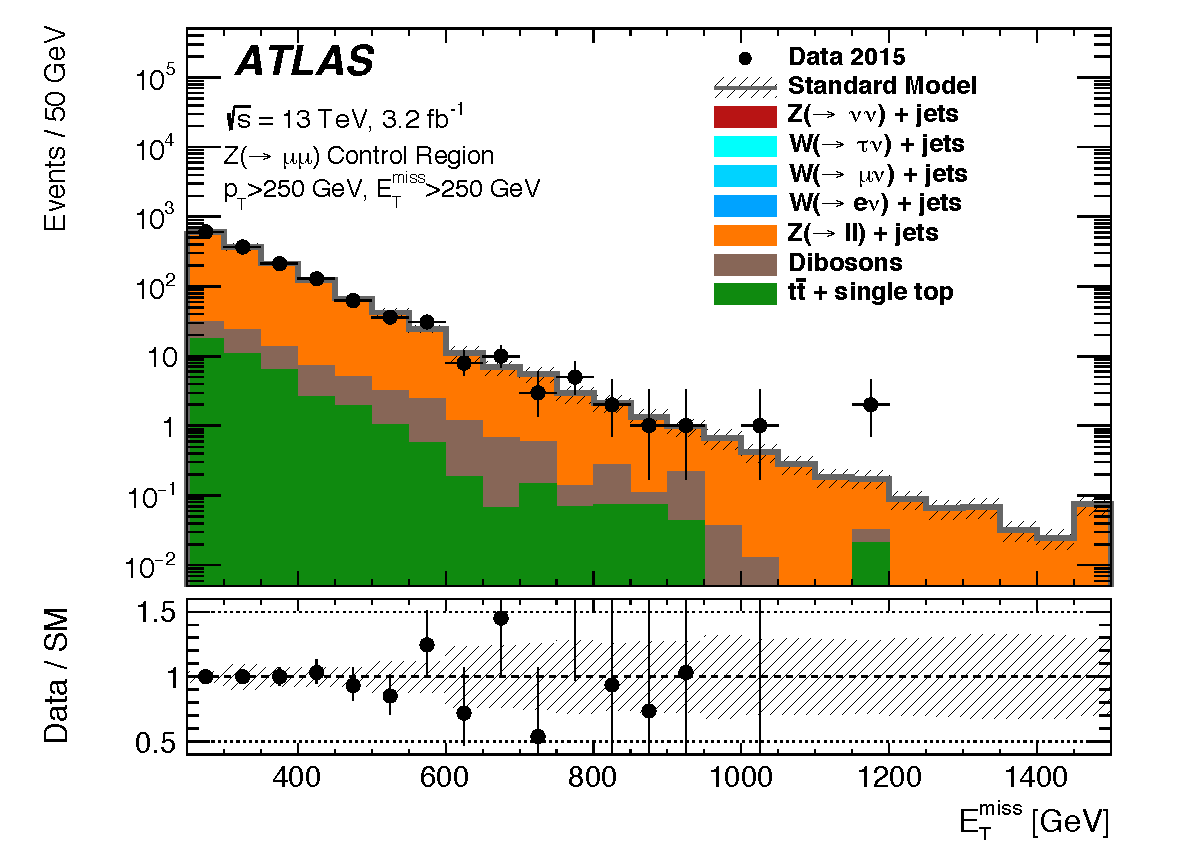
\includegraphics[width=\linewidth]{dimuon_cr_et_miss_post_fit}
    \caption{$\met$ distribution.}
    \label{fig:dimuon_cr_et_miss_pre_fit}
  \end{subfigure}
  \begin{subfigure}[t]{.48\linewidth}
    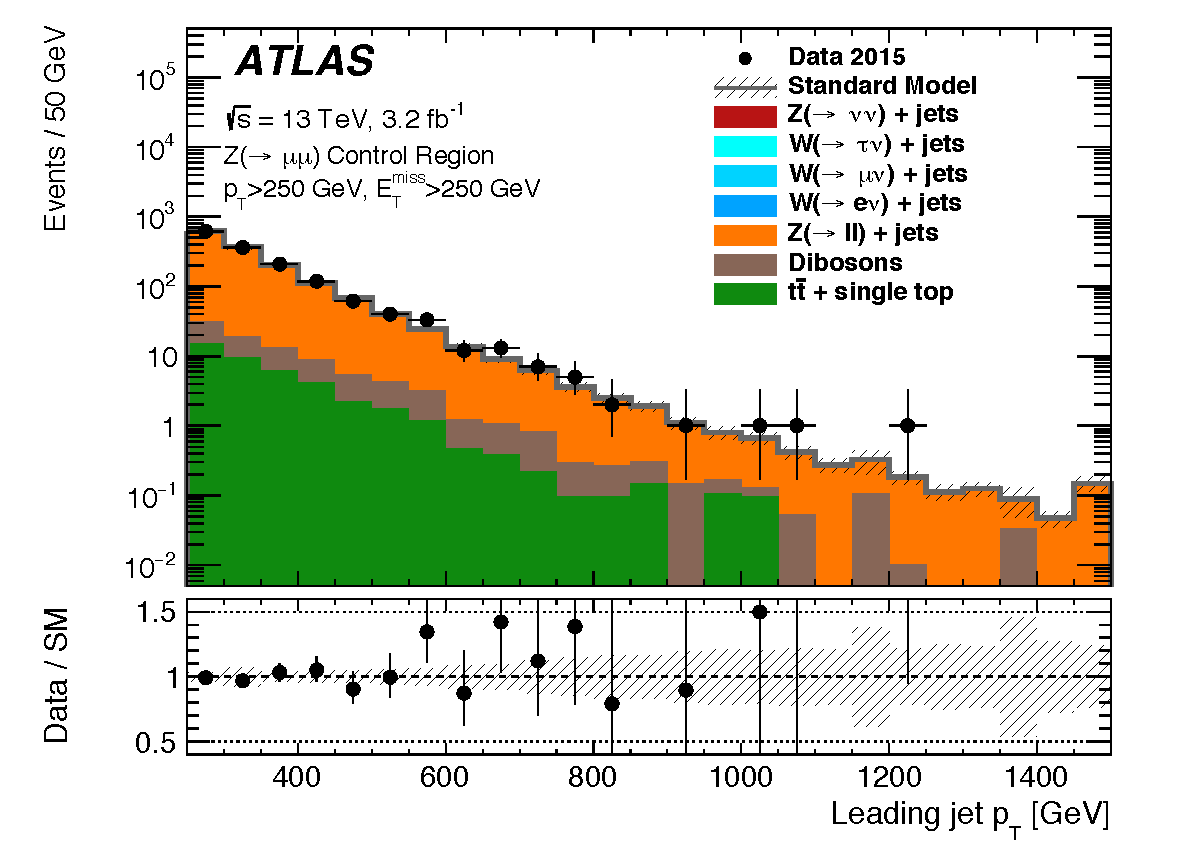
\includegraphics[width=\linewidth]{dimuon_cr_jet1_pt_post_fit}
    \caption{Leading jet $\pt$ distribution.}
    \label{fig:dimuon_cr_jet1_pt_pre_fit}
  \end{subfigure}
  \caption{Observed and predicted $\met$ and leading jet $\pt$ distributions
    after the background only fit in the di-muon $\crzmm$ for the
    $\met > 250~$GeV selection. The error bands include the statistical and
    systematic error.}
  \label{fig:dimuon_cr_plots}
\end{figure}
%%% Local Variables:
%%% mode: latex
%%% TeX-master: "../search_for_DM_LED_with_ATLAS"
%%% End:
